\begin{figure}[h]
	\centering
	
	\begin{tabularx}{\textwidth}{ p{.2\textwidth} | X | X }
		\textbf{Akteur} & \textbf{Beschreibung} & \textbf{Verwendet in Anwendungsfall} \\ \hline
		Nutzer & Bei Nutzern handelt es sich um die Anwender
 der Webanwendung und der App. Hierbei ist keine Authentifizierung erforderlich. Nutzer können sich auf
 den beiden Nutzeroberflächen mittels Verlinkungen zwischen den Haupt- und Teilprojekten bewegen.
 In der Android-App kann ein Nutzer zusätzlich zum reinen Lesen (read-only in Webanwendung) noch
 Teilprojekte bewerten und Kommentare verfassen. & A01, A02, A03, A04 \\ \hline
		Administrator & Der Administrator hat zusätzlich zu den Berechtigungen des Nutzers
 die Möglichkeit, von der Webanwendung aus, Kommentare zu löschen. Das admin-Konto ist dabei vorgegeben
 und die Verwaltung von Benutzeraccounts gehört damit nicht zu den Aufgaben dieses Administrators. & W01, W02
	\end{tabularx}

	
	\caption{Beschreibung der Akteure}
	\label{fig:akteur-tabelle}
\end{figure}


%%%%%%%%%%%%%%%
%% Anwendungsfall 1 %%
%%%%%%%%%%%%%%%
\newpage
\section{Anwendungsfalldiagramme}
Die Anwendungsfalldiagramme haben den Zweck, die Kernfunktionen der Software fur die verschiedenen Akteure zu beschreiben.
\subsection{Anwendungsfalldiagramm - App}

\begin{figure}[h]
	\centering
	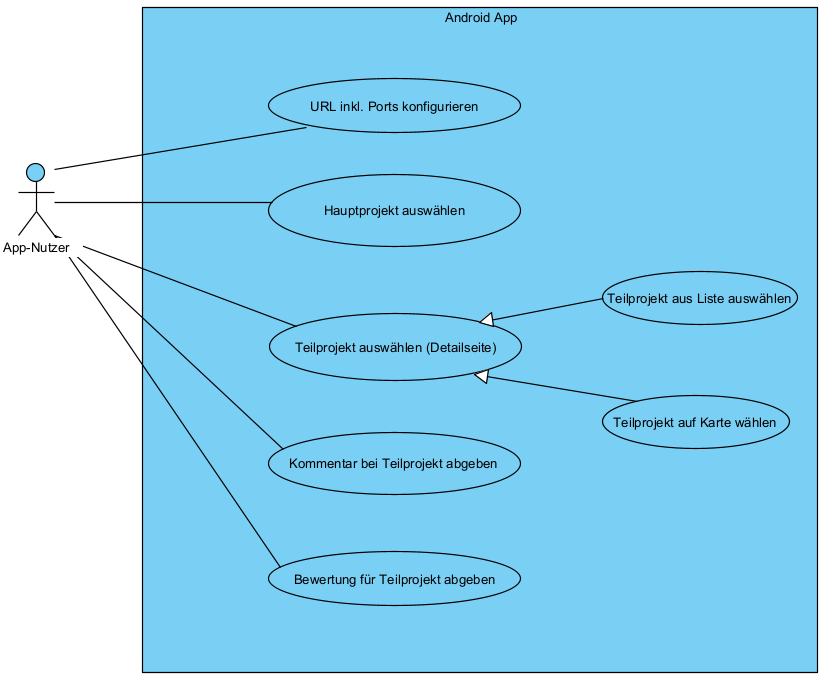
\includegraphics[width=\textwidth]{img/usecaseandroid.png}		
	\caption{Anwendungsfalldiagramm - App}
	\label{fig:anwendungsfalldiagramm-app}
\end{figure}

\newpage

\newpage

%%%%%%%%%%%%%%%
%% Anwendungsfall 2 %%
%%%%%%%%%%%%%%%
\newpage

\subsection{Anwendungsfalldiagramm - Webanwendung}

\begin{figure}[h]
	\centering
	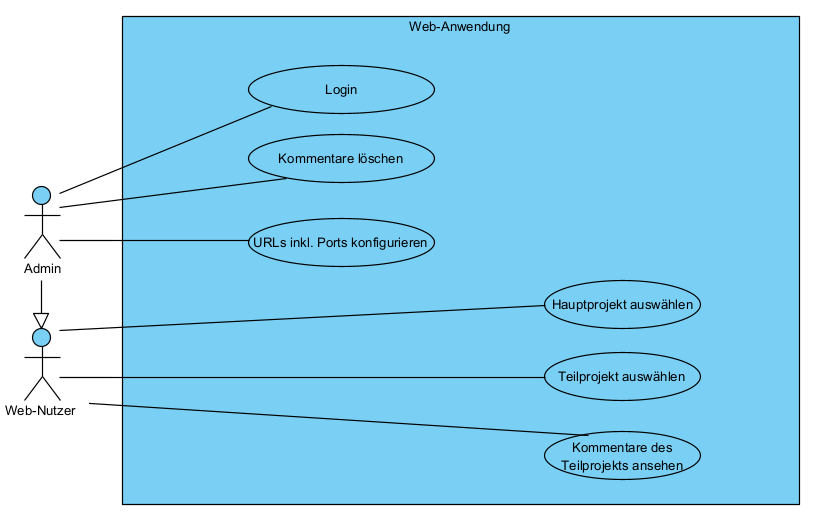
\includegraphics[width=\textwidth]{img/usecaseweb.png}	
	\caption{Anwendungsfalldiagramm - Webanwendung}
	\label{fig:anwendungsfalldiagramm-server}
\end{figure}

\newpage

\section{Anwendungsfälle}
Im Folgendem sind die wichtigsten Anwendungsfälle aufgelistet. Unterstützend stehen Mockups zur Verfügung, um einen Eindruck von der geplanten grafischen Oberfläche zu geben.
\begin{figure}[h]
	\centering
	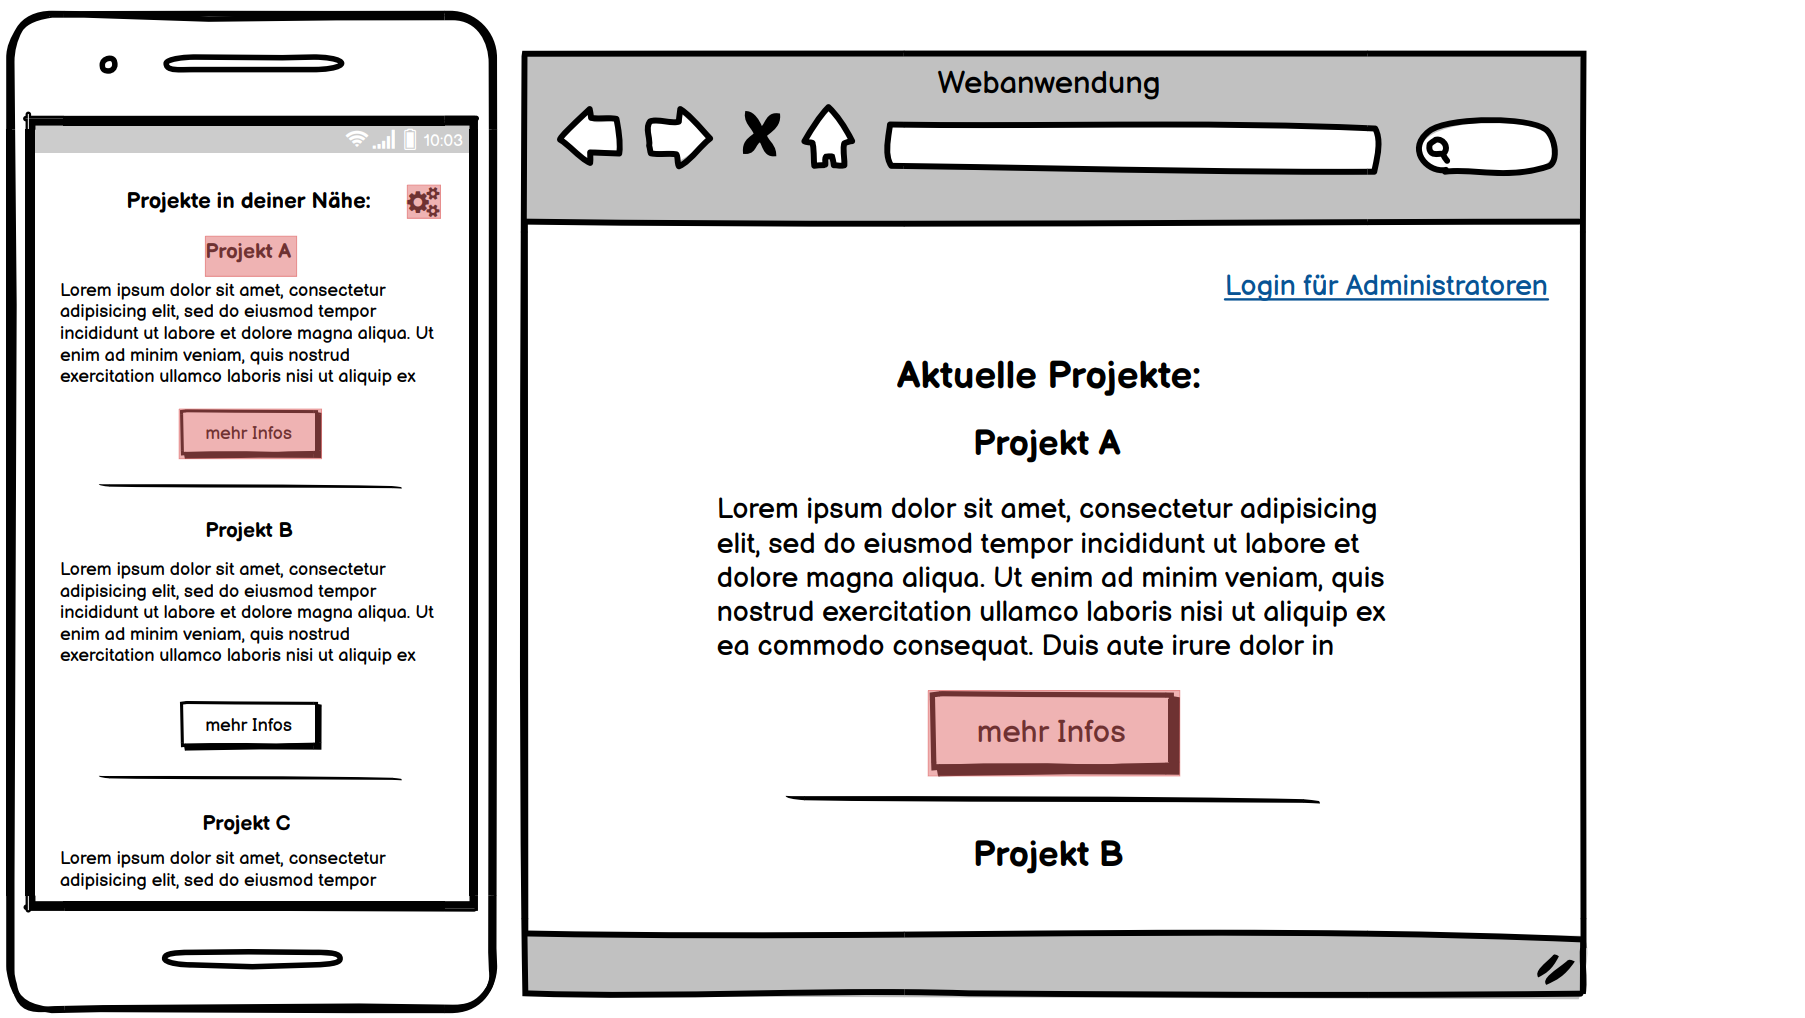
\includegraphics[width=\textwidth]{img/MUstart.png}			
	\caption{Startseite}
	\label{fig:anwendungsfalldiagramm-app}
\end{figure}

\begin{figure}[h]
	\centering
	\begin{tabularx}{\textwidth}{ X | X }
		\textbf{Anwendungsfall ID} & A01 \\ \hline
		\textbf{Anwendungsfallname} & Teilprojekt auswählen (Detailseite) (App, Webanwendung) \\ \hline
		\textbf{Initiierender Akteur} & Nutzer \\ \hline
		\textbf{Kurzbeschreibung} & Der Nutzer wählt ein spezifisches Teilprojekt des jeweiligen Hauptprojektes.  \\ \hline
		\textbf{Vorbedingungen} & Der Nutzer befindet sich auf der Seite eines Hauptprojektes.  \\ \hline
		\textbf{Nachbedingungen} & Der Nutzer befindet sich auf der Detailseite des ausgewählten Teilprojektes.  \\ \hline
		\textbf{Ablauf} &
			\begin{enumerate}
				\item Der Nutzer sucht auf der Seite eines Hauptprojekt ein Teilprojekt aus der nach Entfernung sortierten Liste aus.
				\item Der Nutzer tippt auf das gewünschte Teilprojekt.
			\end{enumerate} \\ \hline
		\textbf{Alternative} &
				\begin{enumerate}
					\item  Der Nutzer wählt das gewünschte Teilprojekt, indem er auf eine Stecknadel auf der eingebetteten Karte tippt.
				\end{enumerate}  \\ \hline
		\textbf{Ausnahme} &
				\begin{enumerate}
					\item Das Hauptprojekt enthält keine Informationen über Teilprojekte.
				\end{enumerate}  \\ \hline
	\end{tabularx}
	\caption{Anwendungsfall A01}
	\label{fig:anwendungsfall-app-tabelle-xx-1}
\end{figure}

\begin{figure}[h]
	\centering
	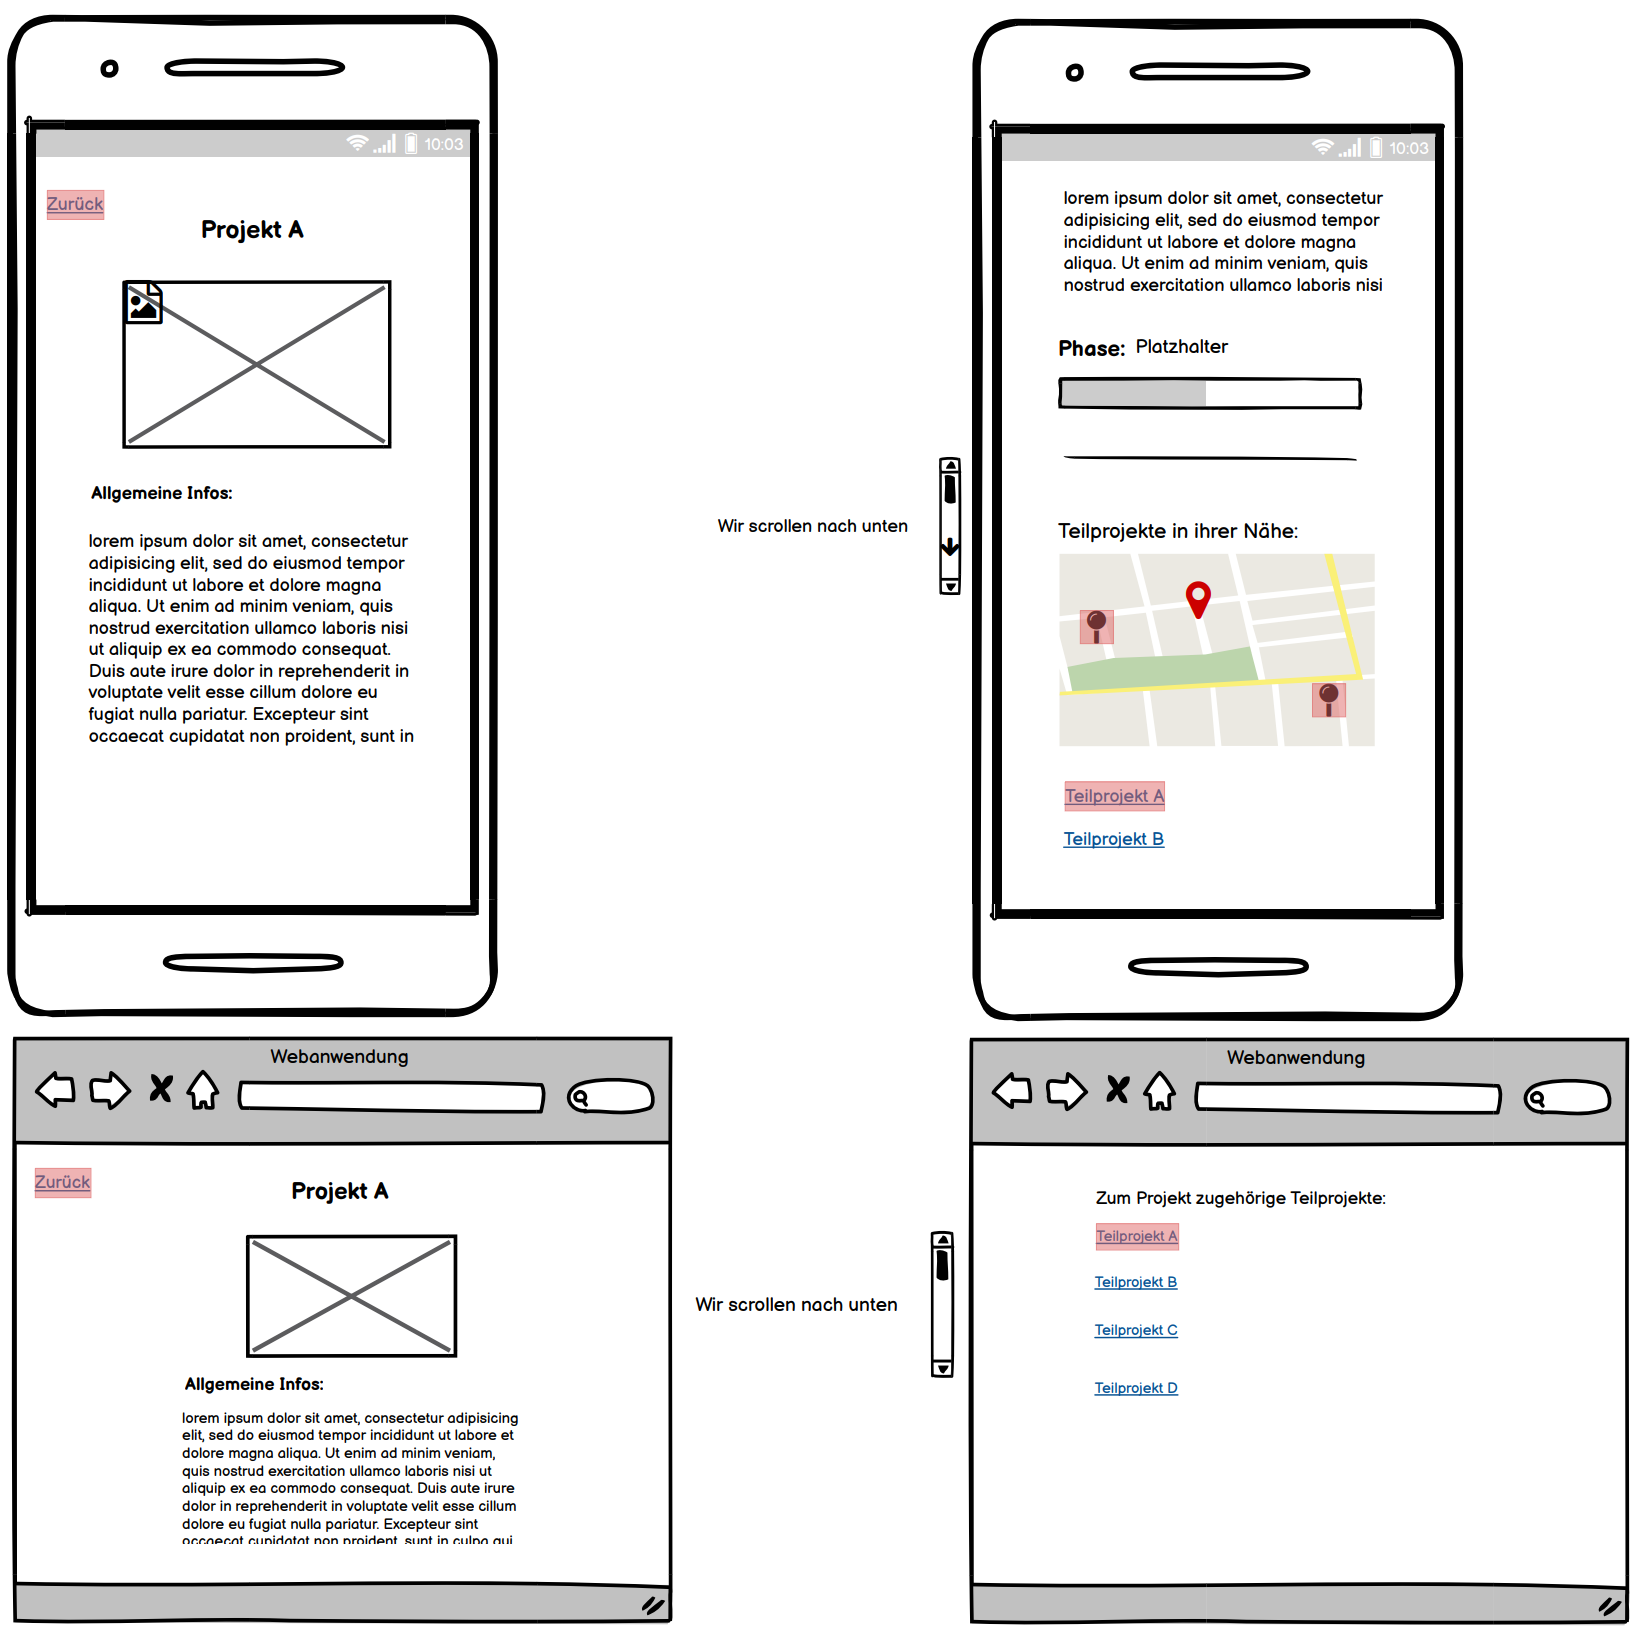
\includegraphics[width=\textwidth]{img/MUhaupt.png}			
	\caption{Auswahl Teilprojekt}
	\label{fig:anwendungsfalldiagramm-app}
\end{figure}


\begin{figure}[h]
	\centering
	\begin{tabularx}{\textwidth}{ X | X }
		\textbf{Anwendungsfall ID} & A02 \\ \hline
		\textbf{Anwendungsfallname} & Kommentar bei Teilprojekt abgeben (App) \\ \hline
		\textbf{Initiierender Akteur} & Nutzer \\ \hline
		\textbf{Kurzbeschreibung} & Der Nutzer gibt einen schriftlichen Kommentar zu einem Teilprojekt ab  \\ \hline
		\textbf{Vorbedingungen} & Der Nutzer befindet sich auf der Detailseite eines Teilprojektes  \\ \hline
		\textbf{Nachbedingungen} & Der Kommentar wird in der öffentlichen Kommentarsektion des Teilprojektes angezeigt, Der Nutzer erhält eine Bestätigung über die Abgabe seines Kommentars.  \\ \hline
		\textbf{Ablauf} &
			\begin{enumerate}
				\item Der Nutzer tippt in das Kommentarfeld und gibt seinen Kommentar ein.
				\item Der Nutzer tippt auf den Button "Absenden".
			\end{enumerate} \\ \hline
		
	\end{tabularx}
	\caption{Anwendungsfall A02}
	\label{fig:anwendungsfall-app-tabelle-xx-1}
\end{figure}

\begin{figure}[h]
	\centering
	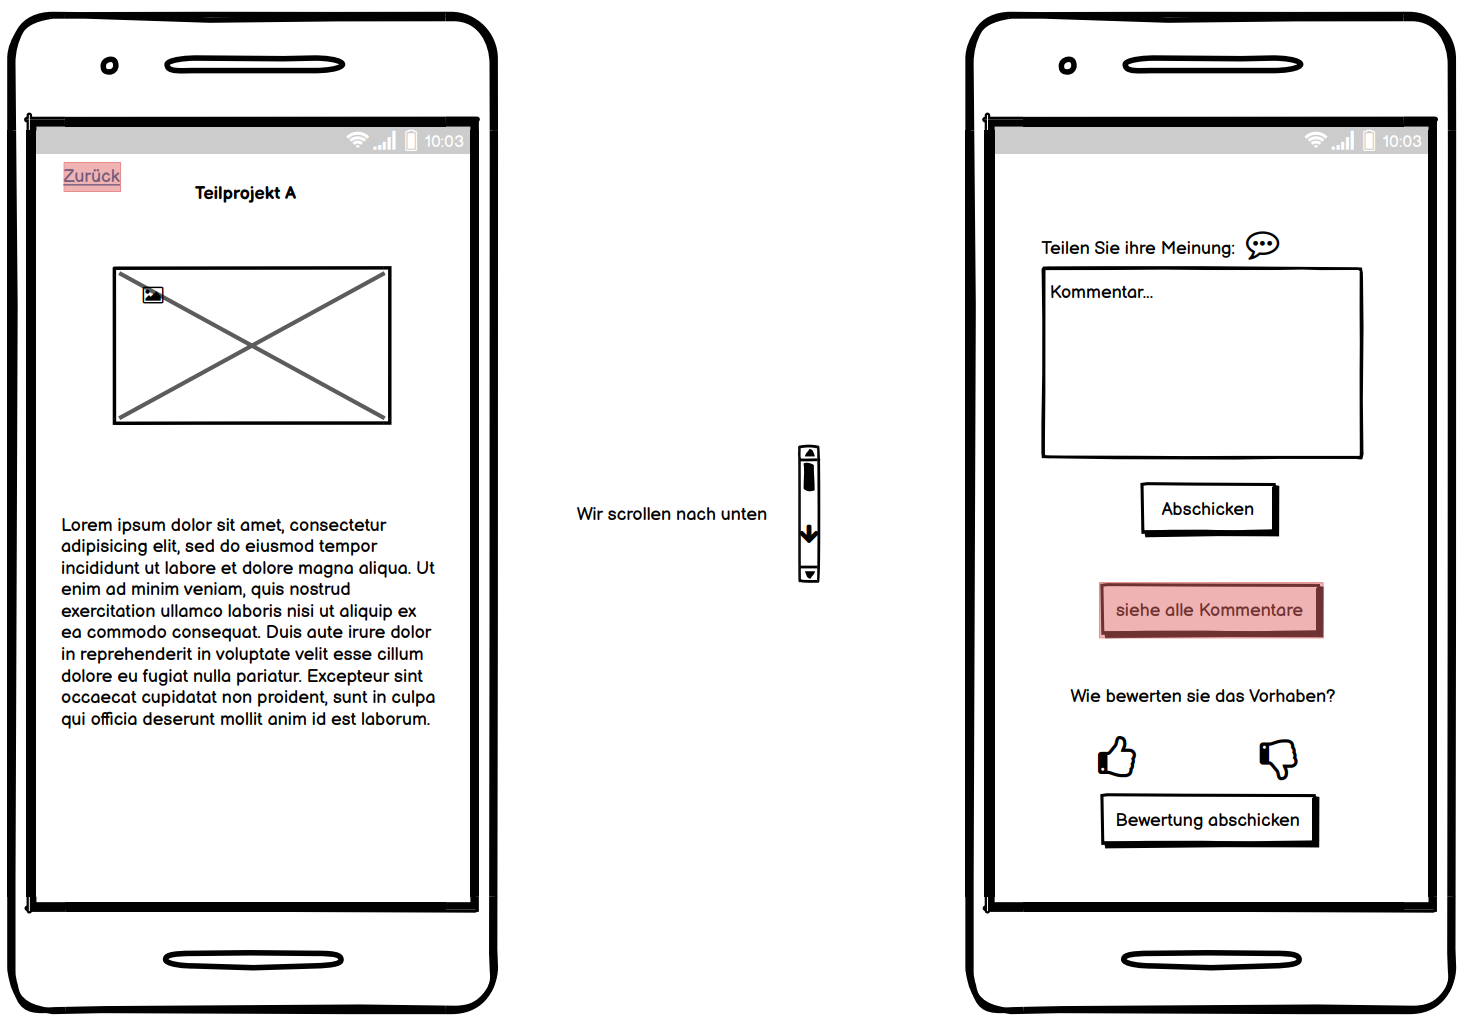
\includegraphics[width=\textwidth]{img/MUcomment.png}			
	\caption{Teilprojekt kommentieren und bewerten}
	\label{fig:anwendungsfalldiagramm-app}
\end{figure}

\begin{figure}[h]
	\centering
	\begin{tabularx}{\textwidth}{ X | X }
		\textbf{Anwendungsfall ID} & A03 \\ \hline
		\textbf{Anwendungsfallname} & Bewertung abgeben (App) \\ \hline
		\textbf{Initiierender Akteur} & Nutzer \\ \hline
		\textbf{Kurzbeschreibung} & Der Nutzer bewertet ein Teilprojekt mittels Daumen.  \\ \hline
		\textbf{Vorbedingungen} & Der Nutzer befindet sich auf der Detailseite eines Teilprojektes.  \\ \hline
		\textbf{Nachbedingungen} & Eine Bestätigung für die Abgabe der Bewertung wird angezeigt (evtl. mit farblicher Hinterlegung des jeweiligen Daumens).  \\ \hline
		\textbf{Ablauf} &
			\begin{enumerate}
				\item Der Nutzer tippt auf den gewünschten Daumen.
			\end{enumerate} \\ \hline
	\end{tabularx}
	\caption{Anwendungsfall A03}
	\label{fig:anwendungsfall-app-tabelle-xx-1}
\end{figure}


\begin{figure}[h]
	\centering
	\begin{tabularx}{\textwidth}{ X | X }
		\textbf{Anwendungsfall ID} & A04 \\ \hline
		\textbf{Anwendungsfallname} & URL inklusive Ports konfigurieren (App) \\ \hline
		\textbf{Initiierender Akteur} & Nutzer \\ \hline
		\textbf{Kurzbeschreibung} & Der Nutzer ändert die URL des Backend-Servers.  \\ \hline
		\textbf{Vorbedingungen} & Der Nutzer befindet sich auf der Einstellungsseite.  \\ \hline
		\textbf{Nachbedingungen} & Ein Bestätigungstext wird angezeigt.  \\ \hline
		\textbf{Ablauf} &
			\begin{enumerate}
				\item Der Nutzer gibt gewünschte URL in das Textfeld ein.
				\item Der Nutzer bestätigt die neue URL indem er auf den Button „Bestätigen“ tippt.
			\end{enumerate} \\ \hline
	\end{tabularx}
	\caption{Anwendungsfall A04}
	\label{fig:anwendungsfall-app-tabelle-xx-1}
\end{figure}

\begin{figure}[h]
	\centering
	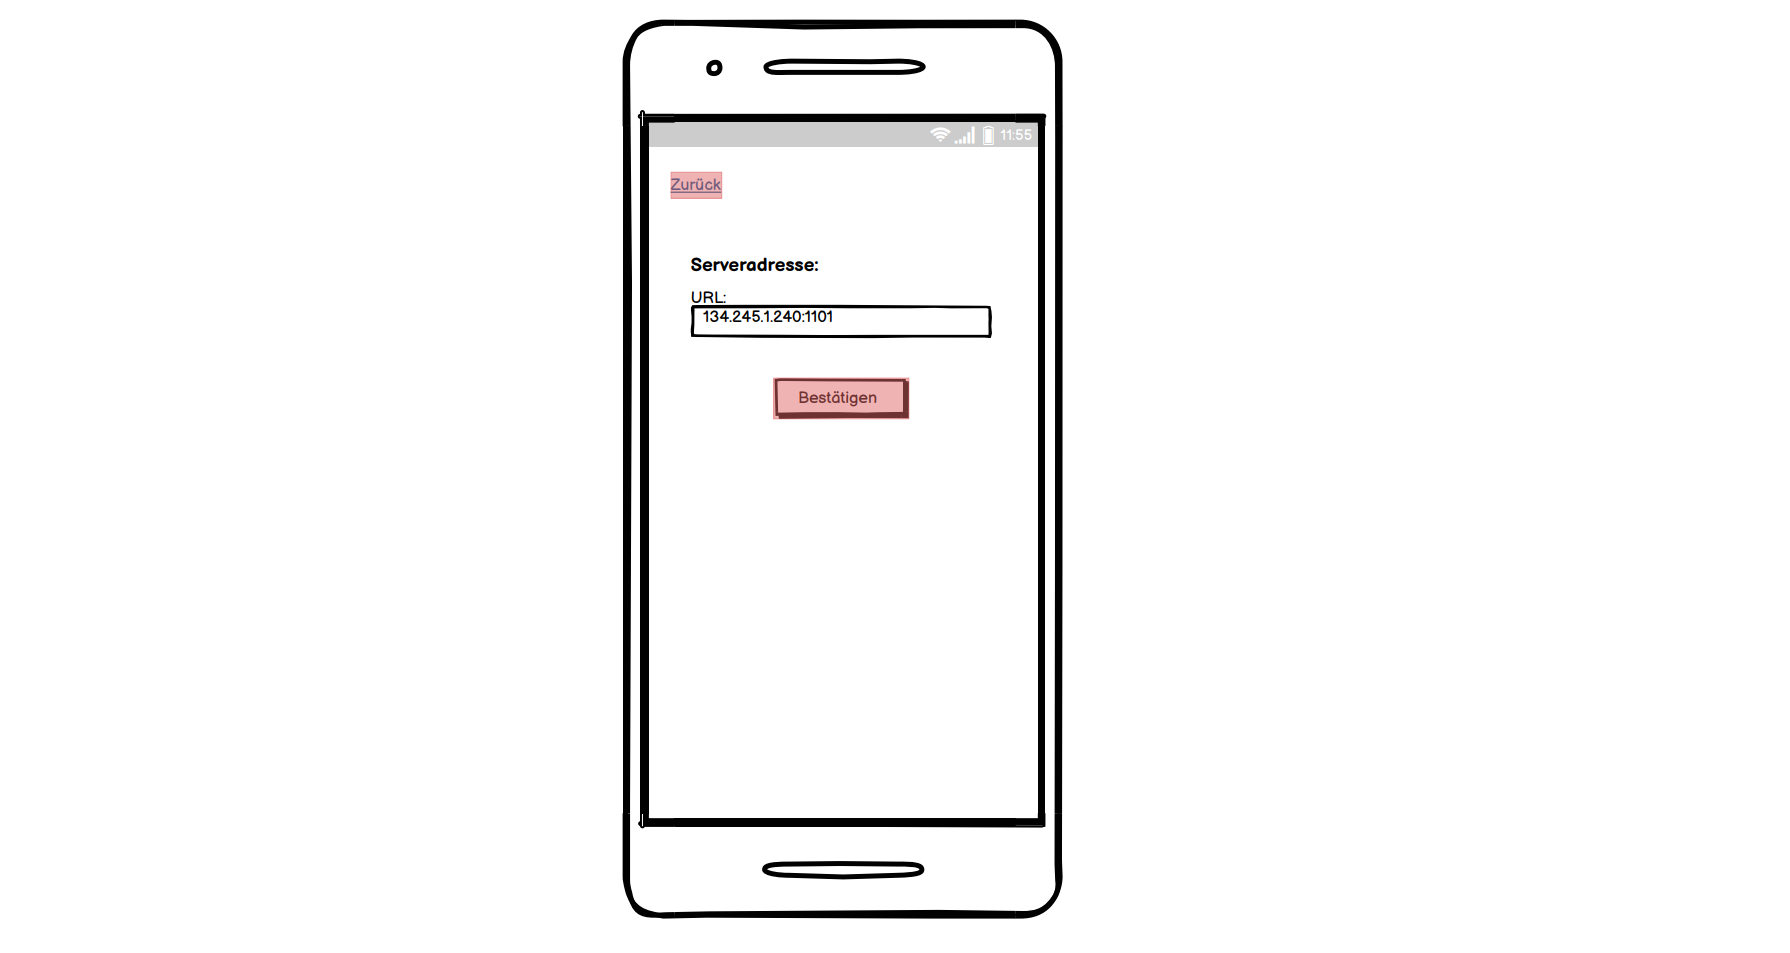
\includegraphics[width=\textwidth]{img/MUurl.png}			
	\caption{URL konfigurieren}
	\label{fig:anwendungsfalldiagramm-app}
\end{figure}


\begin{figure}[h]
	\centering
	\begin{tabularx}{\textwidth}{ X | X }
		\textbf{Anwendungsfall ID} & W01 \\ \hline
		\textbf{Anwendungsfallname} & Kommentar löschen (Detailseite) (App, Webanwendung) \\ \hline
		\textbf{Initiierender Akteur} & Administrator\\ \hline
		\textbf{Kurzbeschreibung} & Der Administrator löscht den gewünschten Kommentar.  \\ \hline
		\textbf{Vorbedingungen} & Der Administrator ist als Benutzer admin eingeloggt. Der Administrator befindet sich auf der Detailseite eines Teilprojektes.  \\ \hline
		\textbf{Nachbedingungen} & Der Text des Kommentars wurde geändert auf „Dieser Kommentar wurde vom Administrator gelöscht.“.  \\ \hline
		\textbf{Ablauf} &
			\begin{enumerate}
				\item Der Administrator wählt Kommentar aus, welcher gelöscht werden soll.
				\item Der Administrator löscht den Inhalt des Kommentars, indem er auf den Button "Löschen" tippt.
			\end{enumerate} \\ \hline
	\end{tabularx}
	\caption{Anwendungsfall W01}
	\label{fig:anwendungsfall-app-tabelle-xx-1}
\end{figure}

\begin{figure}[h]
	\centering
	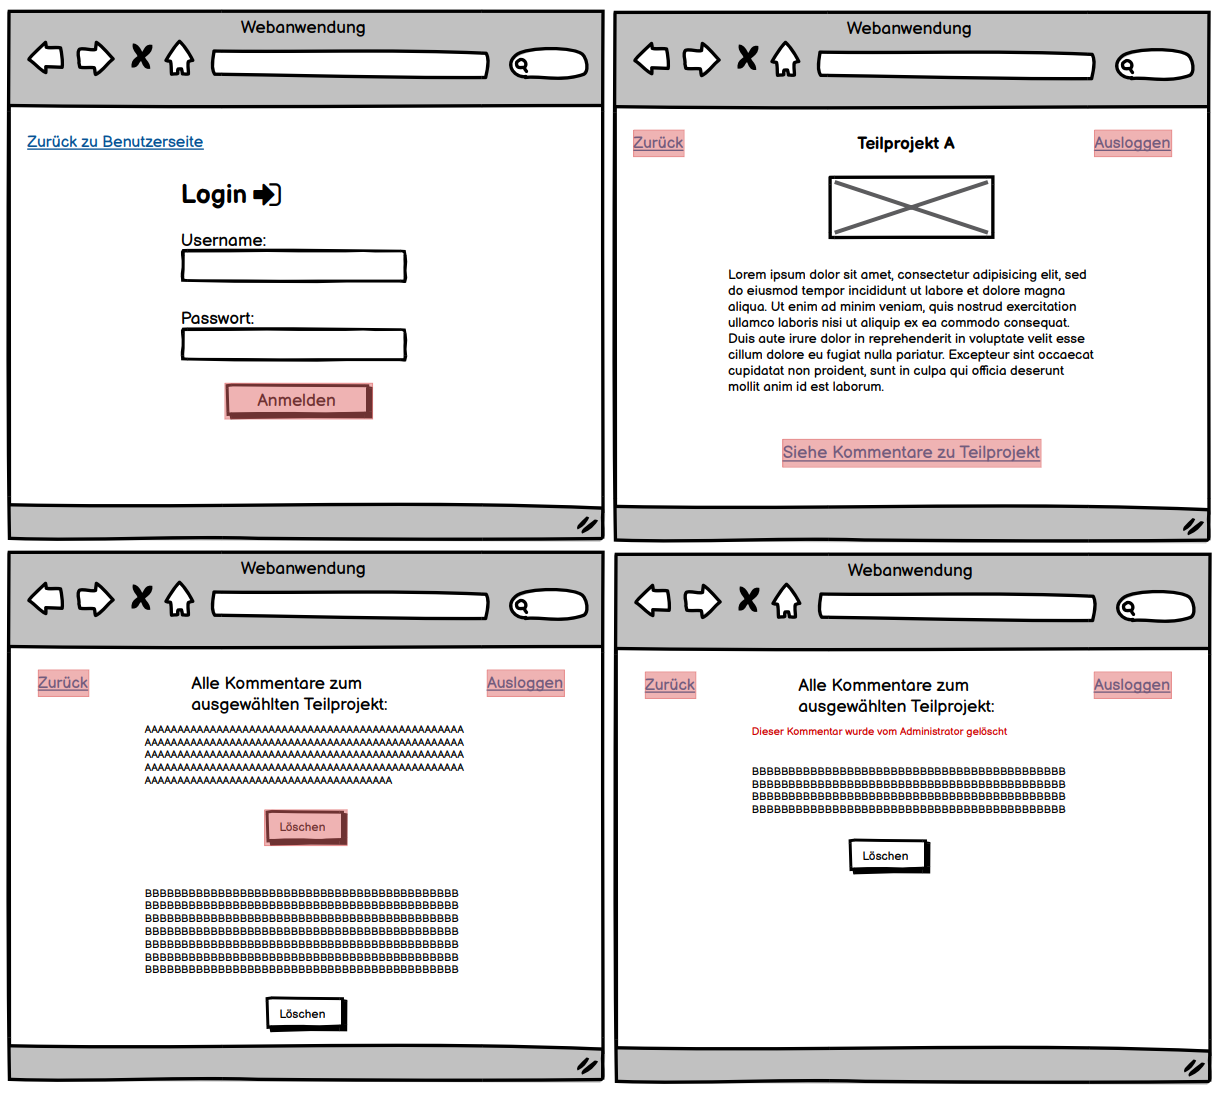
\includegraphics[width=\textwidth]{img/MUdelete.png}			
	\caption{Kommentar löschen}
	\label{fig:anwendungsfalldiagramm-app}
\end{figure}


\begin{figure}[h]
	\centering
	\begin{tabularx}{\textwidth}{ X | X }
		\textbf{Anwendungsfall ID} & W02 \\ \hline
		\textbf{Anwendungsfallname} & URLs inklusive Ports konfigurieren (Webanwendung) \\ \hline
		\textbf{Initiierender Akteur} & Administrator\\ \hline
		\textbf{Kurzbeschreibung} & Der Administrator ändert die URLs der Anwendung für die Datenbank und/oder das Backend  \\ \hline
		\textbf{Vorbedingungen} & Der Administrator ist als Benutzer admin eingeloggt. Der Administrator befindet sich auf der Einstellungsseite.  \\ \hline
		\textbf{Nachbedingungen} & Ein Bestätigungstext wird angezeigt.  \\ \hline
		\textbf{Ablauf} &
			\begin{enumerate}
				\item Der Administrator gibt die gewünschte URL in das jeweilige Textfeld.
				\item Der Administrator bestätigt die neue URL mit einem Klick auf den Button „Bestätigen“.
			\end{enumerate} \\ \hline
	\end{tabularx}
	\caption{Anwendungsfall W02}
	\label{fig:anwendungsfall-app-tabelle-xx-1}
\end{figure}

\begin{figure}[h]
	\centering
	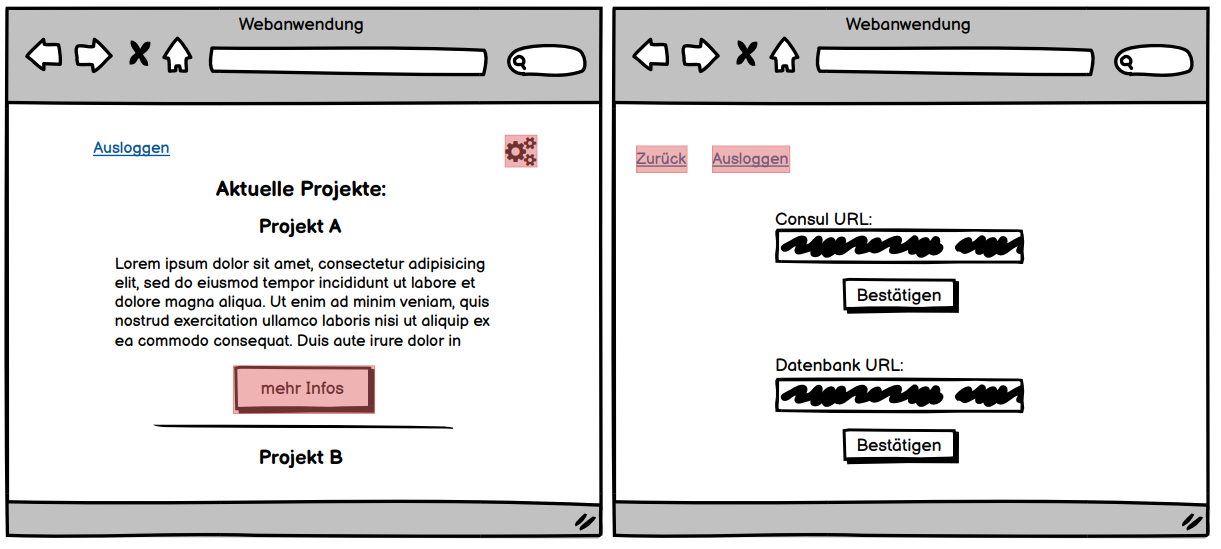
\includegraphics[width=\textwidth]{img/MUurlweb.png}			
	\caption{Backend URL konfigurieren}
	\label{fig:anwendungsfalldiagramm-app}
\end{figure}
